\documentclass{article}[11]
\usepackage{palatino}
\usepackage{graphicx}
\usepackage[colorinlistoftodos]{todonotes}
\usepackage{indentfirst}
\usepackage[]{blindtext}
\usepackage{wrapfig}


\usepackage{float}
\usepackage{graphicx}

\definecolor{dkgreen}{rgb}{0,0.6,0}
\definecolor{gray}{rgb}{0.5,0.5,0.5}
\definecolor{mauve}{rgb}{0.58,0,0.82}

\usepackage{listings}
\lstset{frame=tb,
  language=Java,
  aboveskip=3mm,
  belowskip=3mm,
  showstringspaces=false,
  columns=flexible,
  basicstyle={\small\ttfamily},
  numbers=none,
  numberstyle=\tiny\color{gray},
  keywordstyle=\color{blue},
  commentstyle=\color{dkgreen},
  stringstyle=\color{mauve},
  breaklines=true,
  breakatwhitespace=true,
  keywordsprefix={@},
  tabsize=3
}


%margins as described in "Ghid de redactare Diploma Licenta" by  Mihai Micea
\usepackage[top=1.37in, bottom=1.18in, left=1.18in, right=0.78in]{geometry}

\usepackage[english]{babel}
\usepackage{combelow}
\usepackage[utf8x]{inputenc}

%\useshorthands{'}
%\defineshorthand{'s}{\cb{s}}
%\defineshorthand{'a}{ă}
%\defineshorthand{'t}{\cb{t}}
%\defineshorthand{'S}{\cb{S}}
%\defineshorthand{'T}{\cb{T}}

\usepackage{acro}
\acsetup{first-style=short}

\DeclareAcronym{app}{
	short = app,
	long = application,
	class = abbrev
}

\DeclareAcronym{apps}{
	short = apps,
	long = applications,
	class = abbrev
}

\DeclareAcronym{SDM}{
	short = SDM,
	long = Software Design Methods,
	class = abbrev
}

\DeclareAcronym{OOD}{
	short = OOD,
	long = Object-oriented design,
	class = abbrev
}

\DeclareAcronym{UML}{
	short = UML,
	long = Unified Modeling Language,
	class = abbrev
}

\DeclareAcronym{DP}{
	short = DP,
	long = Design Patterns,
	class = abbrev
}

\DeclareAcronym{OOP}{
	short = OOP,
	long = Object-oriented programming,
	class = abbrev
}

\DeclareAcronym{MVP}{
	short = MVP,
	long = Model View Presenter,
	class = abbrev
}

\usepackage{hyperref}
\hypersetup{
    colorlinks=true,
    linkcolor=blue,
    filecolor=magenta,      
    urlcolor=cyan,
    citecolor=blue}

\begin{document}



\begin{titlepage}

\newcommand{\HRule}{\rule{\linewidth}{0.5mm}} % Defines a new command for the horizontal lines, change thickness here

\center % Center everything on the page
 
%----------------------------------------------------------------------------------------
%	HEADING SECTIONS
%----------------------------------------------------------------------------------------

\textsc{\LARGE Universitatea "Politehnica" Timi\cb{s}oara}\\[1.5cm] % Name of your university/college
\textsc{\Large Course: Software Project Management}\\[0.5cm] % Major heading such as course name

\vspace{3cm}


%----------------------------------------------------------------------------------------
%	TITLE SECTION
%----------------------------------------------------------------------------------------

\HRule \\[0.4cm]
{ \huge \bfseries %
		HelpMeSee\\ \Large
		Mobile personal assistant application for visually impaired people\\
		Project: Software Design Methods
}\\[0.4cm] % Title of your document
\HRule \\[1.5cm]
 
%----------------------------------------------------------------------------------------
%	AUTHOR SECTION
%----------------------------------------------------------------------------------------

\begin{minipage}{0.4\textwidth}
\begin{flushleft} \large
\emph{Author:}\\
Marius \textsc{Olariu} % Your name
\end{flushleft}
\end{minipage}
~
\begin{minipage}{0.4\textwidth}
\begin{flushright} \large
\emph{Lecturer:\hspace{2cm}} \\
Dr. Răzvan \textsc{Cioargă} % Supervisor's Name
\end{flushright}
\end{minipage}\\[2cm]

% If you don't want a supervisor, uncomment the two lines below and remove the section above
%\Large \emph{Author:}\\
%John \textsc{Smith}\\[3cm] % Your name

%----------------------------------------------------------------------------------------
%	DATE SECTION
%----------------------------------------------------------------------------------------



%----------------------------------------------------------------------------------------
%	LOGO SECTION
%----------------------------------------------------------------------------------------
\vspace{3.5cm}


\includegraphics{./imgs/UptLogo.jpg}\\[1cm] % Include a department/university logo - this will require the graphicx package
 
%----------------------------------------------------------------------------------------

\vfill % Fill the rest of the page with whitespace

\end{titlepage}

\tableofcontents
\newpage

\section{Description of the project}
	Nowadays software runs the world but most of the software solutions are designed for healthy people. Thus,  the visually impaired people are somehow left aside. However, recently things have begun to change and since everyone now owns a smartphone, there have been developed a series of apps for the visually impaired people. Most successful apps are \emph{Be My Eyes} (establishes a live video connection with an volunteer that describes the surroundings to the blind person), BeSpecular(the visually impaired person takes a photo, attaches a voice message to it and sends it to a volunteer that provides help) or the most helpful (in my opinion) \emph{Seeing Ai} from Microsoft. The later \ac{app} is an assistant which is able to recognize "saved" persons and describe their emotions, read text aloud from labels/books etc., provide description of images from other \ac{apps} (e.g. Facebook) by importing them into \emph{Seeing Ai} or scene description. However, it is developed only for \emph{iOS}. The other apps in this sector have a free and limited variant and in order to make use of all the features the user has to purchase it. \\
	
	To address the above mentioned drawbacks an app should be developed for this sector, namely \emph{HelpMeSee}. This app should be an mobile personal assistant  that will offer a different perspective compared to what's on the market at this point. If this app will be a success then
	
	%TODO add logo of the app
	
	\newpage

\section{Requirements}

\subsection{Functional requirements}

\subsubsection{Directions}
	The app should provide assistance to the blind user when he/she tries to get to a location. The user will be guided using spoken descriptions (e.g. "Go straight 100 meters", "You are about to cross the street").
	
\subsubsection{Location}
	The user can ask the app to retrieve his current location (e.g. "Bld. Industriei, nr. 6) and has the possibility to share his current location to a list of predefined friends.
	
\subsubsection{Scene description}
	By taking a photo the user is able to obtain information about his/her surroundings (e.g. "A red car is parked in front of you.") and this phrase will be read out loud.
	
\subsubsection{Text recognition}
	The app should be able to recognize text and read it out loud. The sources of text could be: text written on paper, labels on products or handwritten notes.
	
	
\subsection{Nonfunctional requirements}

\subsubsection{Usability}
	There must be designed mechanisms that allow the users to navigate through app and access its features easily given their condition.

\subsubsection{Maintainability}
	Due to the fact that bugs are inevitable the implementation of the app must adhere to \textbf{O}bject \textbf{O}riented \textbf{D}esign \textbf{P}rinciples (e.g. \textbf{S}ingle Class Responsibility, \textbf{O}pen-close, \textbf{L}iskov substitution, \textbf{I}nterface segregation, \textbf{D}ependency inversion - SOLID) and goals (loose coupling, high cohesion) so that the time spent fixing bugs will be reduced. 


\subsubsection{Extensibility}
	Based on the feedback received from users the app can be extended with new features without great effort. Thus, the architecture of the app must be chosen carefully.


\section{Specifications}

\subsection{Directions}
	In order to implement this part the app will use \emph{Google Directions API} that will provide the fastest walking route from A to B. The fastest route is provided in json file having a certain format. The user is notified from 20 to 20m with spoken instructions about the itinerary.

\subsection{Location}
	Again, \emph{Google Directions API} and the \textbf{G}lobal \textbf{P}ositioning \textbf{S}ystem (GPS) of the phone will be used to retrieve the location of the user. The location is displayed on the phone and read aloud. Also, using the voice command "friends" the app will send user's location to a list of predefined friends using the \textbf{S}hort \textbf{M}essaging \textbf{S}ervice(SMS). To add a friend in this list the user should use the voice command "add friend" followed by the name of the friend and his/her phone number.
	
\subsection{Scene description}
	\emph{Microsoft Cognitive Services} provides \emph{Computer Vision API} that can be used to distill actionable information from images. Therefore, the user takes a photo and then the app will communicate using \textbf{Re}presentational \textbf{S}tate \textbf{T}ransfer (REST) with Microsoft cloud servers to get the description of the image.
	
\subsection{Text recognition}
	The same \emph{Computer Vision API} can be used to detect and extract text from an image.
	
\subsection{Usability}
	Each screen of the app will have a button in the bottom-right corner, the "speech input" button. Thus, the user has the possibility to access a feature without having to navigate between the screens. For example if the user is currently walking to a destination but at some point decides to get info about surroundings, he takes a photo - gets the description, and then continues the journey - all this without leaving the directions screen and not being force to abandon one activity in order to perform another.\\
	
	The widgets size will be slightly bigger than for a normal app. Also, for a simple \emph{tap} the widget name will be spoken out loud and for \emph{double-tap} the widget functionality will be accessed.

\subsection{Maintainability}
	There will be implemented a series of design patterns known for their  positive effect on this maintainability alongside good coding practices (e.g comments, descriptive attributes/methods/class names, reduced size methods etc.). The Factory Method will be used in order to reduce coupling between client classes(e.g. Controller/Presenter classes from Model-View-Presenter architecture) and those which communicate with the cloud services. \\
	
	For accessing each subsystem (i.e. directions, locations, scene description, text recognition) the Facade combined with Singleton pattern will be used. By doing so we do not need to reimplement the functionality of the "speech input" button (present in each screen), thus no code duplication. Also the Facade pattern will allow us to modify the subsystems without having to worry where they are used (since the access to them is through the Facade).
	
\subsection{Usability}
	The architecture for \emph{HelpMeSee} is going to be \textbf{M}odel \textbf{V}iew \textbf{P}resenter (MVP). All the subsystems that communicate with the network and implement business logic will be a part of the \emph{model}. A \emph{view} will contain just the mappings between the UI elements and the objects that control them (no logic is added, for example handling user input actions). The purpose of the a view(screen) is just to display data and notify the \emph{presenter} about user's actions. Next, each \emph{view} will have a presenter, i.e. a interface, that will interact with the model in order to bring data to the view, modify the state of the model and to apply the UI logic.

 
\begin{figure}[H] 
	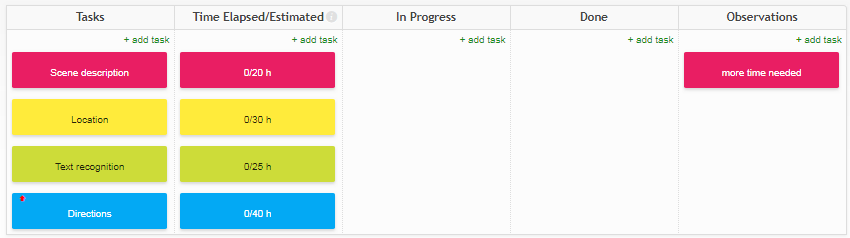
\includegraphics[width=16.5cm,height=8cm]{./imgs/taskSched}
	\caption{Tasks board}
\end{figure}

\section{Software Design Methods}
	\emph{\textbf{S}oftware \textbf{D}esign \textbf{M}ethods} (SPM) guide the software engineer in transforming the requirements into an executable software system. They offer theoretical foundations and at the same time some degree of freedom to innovate. However, there is no "silver bullet" \cite{brooks1987no} or one-size-fits-all for a complex software system.
According to Sommerville\cite{sommerville2010software} the \ac{SDM} can categorized in:

%TODO you can add more about reasons to use SDM to fill space SD-c8

	\begin{itemize}
		\item Top-down structured design
		\item Data-driven design
		\item \textbf{O}bject-\textbf{o}riented \textbf{d}esign (OOD)
	\end{itemize}

	Due to the fact that for this project we use an \textbf{O}bject-\textbf{O}riented paradigm for developing software we will discuss only the OOD methods applied for \emph{HelpMeSee}, that is:
	
	\begin{itemize}
		\item \textbf{U}nified \textbf{M}odeling \textbf{L}anguage (UML)
		\item  \textbf{D}esign \textbf{P}atterns (DP)
		\item \textbf{M}odel-\textbf{V}iew-\textbf{P}resenter (MVP) architecture
	\end{itemize}
	

\newpage

\subsection{Theoretical Background}

	\subsection{Model-View-Presenter}
	
	\begin{wrapfigure}{r}{0.6\textwidth}
		\centering
		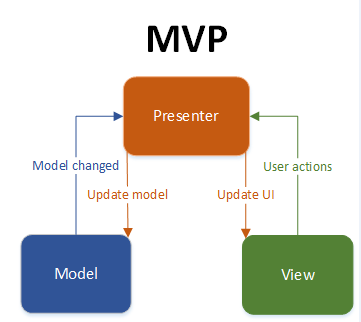
\includegraphics{./imgs/MVP}
		\caption{MVP architecture \cite{MVPPhoto}}
	\end{wrapfigure}
	
	 By using the \ac{MVP} architecture we maximize the code that can be tested with unit tests, separate business logic from UI (thus we adhere to OOP goals of low coupling, high cohesion or \emph{Single Responsability Principle}).  This architecture is based on three types of classes: Model, View and Presenter. The \emph{Model} is responsible for business logic and state of persisted data, \emph{View} for rendering UI elements and the \emph{Presenter} works like a glue between the two (i.e. changes the model data state, fetches data to \emph{View}).\\
	
	 In particular for Android development, we will not end up with huge \emph{Activity} classes (they represent screens). Very often Android programming beginners end up with big Activity classes since there is not a clear distinction if such a class is an UI element or a business logic class, however, we will not detail further on this issue.
	
	\subsection{Unified Modeling Language}
	According to Martin Fowler \cite{fowler2004uml} \ac{UML} "is a family of graphical notations [...] that help in describing and designing software systems, particularly software systems built using the object-oriented (OO) style". From this family of diagrams we will be using only \emph{Class Diagrams}  and \emph{Use Cases}. Class Diagrams represent "the types of objects in system and the various [...] relationships that exist among them" . In the requirements  part we have used \emph{Use Cases} to capture the functional requirements of the app.
	\subsection{Design Patterns}
	Design patterns represent common used solutions to commonly occurring  problems when developing OO software systems. In other words, a DP is a template for how to solve a software problem.
	\subsubsection{Facade}
	\subsubsection{Factory Method}
	\subsubsection{Singleton}

\subsection{Concrete application of the SDM}

\printacronyms[include-classes=abbrev,name=Abbreviations]

%style
\bibliographystyle{ieeetran}

%the place where references will appear in output pdf
\bibliography{SPMBib}

\end{document}